\chapter{Computational studies of Diphtheria Toxin T Domain: role of acidic residue E362 in membrane-protein insertion and pore formation.} \label{DTT}
\small{Authors: Nathan M. Lim, J. Alfredo Freites, Linh P. Nguyen, Douglas J. Tobias, David L. Mobley}\\
\emph{Excerpt from: `Refining Protein Penetration into the Lipid Bilayer Using Fluorescence Quenching and Molecular Dynamics Simulations: The Case of Diphtheria Toxin Translocation Domain' \cite{Kyrychenko2018}}\\
\emph{J. Mem. Bio., 2018, 251 (9), pp 379--391 \\
\doi{doi:10.1007/s00232-018-0030-2}\\Publication Date (Web): March 17, 2018}


\begin{figure}[H]
\centering
\frame{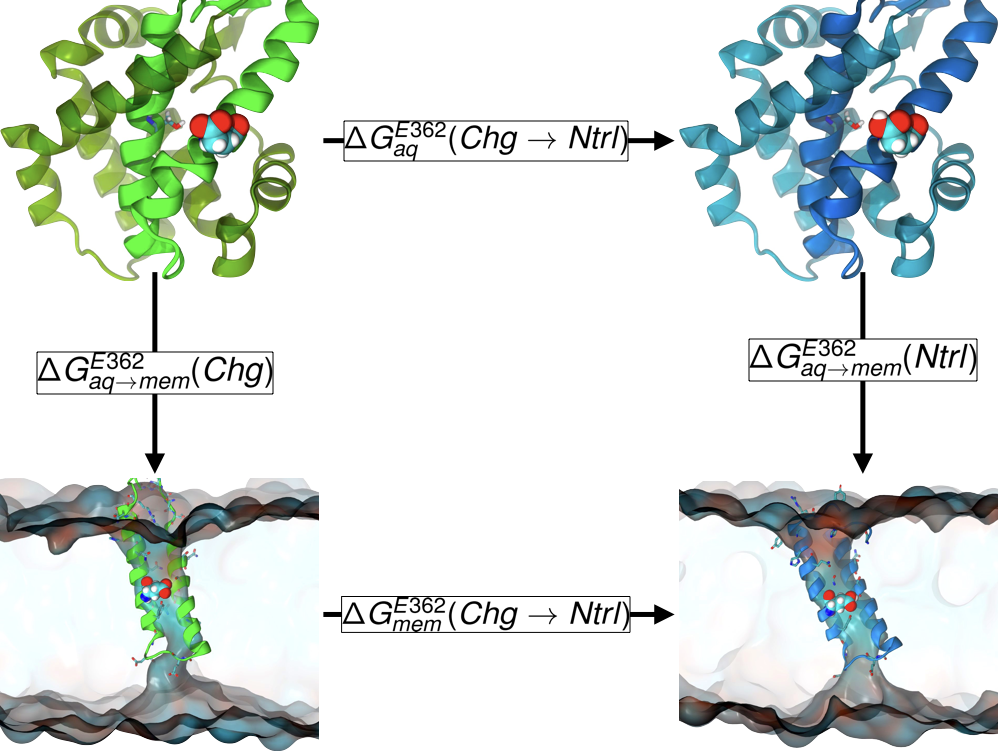
\includegraphics[width=\linewidth,]{Figures/DTT/thermo_cycle.png}}
\caption[Thermodynamic cycle for membrane-protein insertion]{Thermodynamic cycle for calculating membrane-protein insertion free energies of DTT for neutralized E362 relative to charged E362. The vertical legs relate to the membrane insertion free energies of DTT which is obtained from the equivalent horizontal legs calculated from the alchemical free energy calculations. Residue E362 is represented with van der Waals spheres in each image. For figures of the protein, the TH8-TH9 helices are shaded differently from the rest of the protein and S336 is displayed to illustrate its position on the TH8 helix relative to E362.}
\label{fig:dtt_thermo_cycle}
\end{figure}


\section{Introduction}
Recent experimental studies on the Diphtheria Toxin T domain (DTT) characterized the importance in protonation of acidic residue E362 in the membrane insertion process \cite{ghatak2015role}.
Through mutagenesis studies of E362Q--whereby the charge is effectively removed--it was demonstrated that this residue plays a key role in the insertion of the TH8-TH9 helices.
In order to quantitatively understand the role of the charged residue E362 and the energetics in the insertion mechanism of DTT, we compute the membrane-protein insertion free energy.
In this study, we utilize an all-atom (explicit solvent \& membrane) molecular dynamics (MD) simulation with the alchemical free-energy perturbation (FEP) approach.
Here, we compute the change in free energies between the charged and neutral states of E362 from simulations carried out in solution and membrane environments.
Our free energy predictions indicate high favorability (approximately -6$\frac{kcal}{mol}$) for neutral E362 in the membrane-protein insertion pathway--which seems consistent with experimental mutagenesis results \cite{ghatak2015role}.
Additional profiling of the pore formed by DTT indicates neutralized E362 induces larger perturbations to the membrane, providing further evidence E362 plays a key role during insertion.

\section{Methods}
\subsection{Molecular Dynamics simulation \& Free energy calculation protocols}
The initial protein configurations were based on the crystal structure of wild-type diphtheria toxin (PDB ID 1f0l). 
The protein in the solution simulation system consisted of the full T domain (residues 202–378), and in the membrane system, of the TH8–TH9 hairpin (residues 319–380). 
TH8 is a hydrophobic helix while TH9 exhibits a significant hydro- phobic moment. 
In the crystal structure TH8 appears fully protected by the rest of the T domain, therefore, in order to produce an initial protein configuration with favorable interactions with the membrane environment, we rotated TH9 180° about its principal axis so as to orient the polar face towards TH8 and away from the lipid bilayer hydrocarbon core.
Titratable side chains were modeled consistent with neutral pH in the solution system, and with acidic pH in the membrane system. 
Specifically, in the solution system, all histidine residues were neutralized and acidic residues were ionized. 
In the membrane system, all histidine residues were charged and, except for E362, all acidic residues were neutralized. 
The solution simulation system was generated using VMD \cite{humphrey1996vmd}. 
The final solution system consisted of one T domain, 2768 waters and, 10 counterions for a total of 11,032 atoms. 
The membrane system was set up by inserting the TH8–TH9 hairpin in a 1:1 POPC–POPG bilayer in excess water using the CHARMM–GUI membrane builder \cite{jo2009charmm} and VMD. 
The final mem- brane system consisted of one TH8–TH9 hairpin, 250 lipids, 11,724 waters, and 122 counterions for a total of 68,872 atoms. 
Equilibration simulations were carried out at con- stant pressure (1 atm) and temperature (300 K) for approximately 40 and 113 ns for the aqueous and membrane systems, respectively.

The simulations were run with the NAMD (v2.11) software package \cite{phillips2005scalable} under three-dimensional periodic boundary conditions (PBC). 
The protein was modeled using the CHARMM22 force field \cite{mackerell1998all}
The CHARMM36 force field was used for lipids \cite{klauda2010update} and the TIP3P \cite{jorgensen1983comparison} model was used for water. 
A reversible multiple-time- step algorithm \cite{grubmuller1991generalized} was used to integrate the equations of motion with a time step of 4 fs for the long- range electrostatic forces, and 2 fs for the short-range non- bonded forces and the bonded forces. 
The smooth particle mesh Ewald method \cite{essmann1995smooth} was used to calculate electrostatic interactions. 
The short-range interactions were cutoff at 12 Å using a force-based switching scheme.
All bond lengths involving hydrogen atoms were held fixed using the SHAKE \cite{ryckaert1977numerical} and SETTLE \cite{miyamoto1992settle} algorithms. 
A Langevin dynamics scheme was used for thermostating. Nosé–Hoover–Langevin pistons were used for pressure contro (\cite{feller1995constant};\cite{martyna1994constant}).

Alchemical free energy calculations were divided into 40 equally spaced windows with production simulations running for 5 ns per stage, giving a total of 200 ns for each system.
Each production run was preceded by an equilibration protocol consisting of 10,000 steps of conjugate-gradient energy minimization and a 1 ns MD run. 
Free energies were calculated using Bennett Acceptance Ratio \cite{bennett1976efficient} as implemented by the PyMBAR program \cite{shirts2008statistically, chodera2007use}.
Corrections to the final free energies were performed using a scheme based on a continuum-electrostatics analysis, which corrects for spuri- ous interactions encountered when simulations are carried out with periodic boundary conditions \cite{rocklin2013calculating}.

Trajectory analyses were performed using VMD and MDtraj \cite{mcgibbon2015mdtraj}.
Molecular graphics were generated using VMD \cite{humphrey1996vmd}.
Analysis of the pore resulting from the TH8–TH9 hairpin insertion in the membrane was done using dxTuber (v0.28) \cite{raunest2011dxtuber}.
OpenDX density maps were generated using the VolMap(v1.1) plugin in VMD with the following settings: resolution: 1.0 Å atom size: 1.0 × radius, weights: mass
Density maps were combined over the final 64 ns from the membrane MD simulations.
For analysis with dxTuber, we used a combination of two settings: (1) time-averaged for both the protein and solvent and (2) minimum protein density and time-averaged solvent density. Trajectory frames were aligned by the hairpin backbone using the starting frame as reference and then wrapped about the hairpin’s center of mass using MDtraj \cite{mcgibbon2015mdtraj}.

\section{Results \& Discussion}

\begin{table}[H]
\centering
\caption[Initial and corrected free energies]{Initial and corrected\cite{rocklin2013calculating} free energies obtained from alchemical free energy calculations which transformed E362 from charged to neutral in both the aqueous and membrane environments. The membrane-protein insertion free energies are obtained from the difference in free energies between the two environments.}
\label{tbl:dtt_ddG}
\begin{tabular}{|c|c|c|}
\hline
& \boldmath$\Delta G\frac{kcal}{mol}$   & \boldmath$\Delta G\frac{kcal}{mol}$ Corrected     \\ \hline
$\Delta G_{mem}^{E362}(Chg\rightarrow Ntrl)$ & 84.4 & 93.3 (+/- 0.3) \\ \hline
$\Delta G_{aq}^{E362}(Chg\rightarrow Ntrl)$  & 86.0 & 99.5 (+/- 0.2) \\ \hline
$\Delta\Delta G_{aq\rightarrow mem}^{E362}(Ntrl)$ & -1.6 & -6.2 (+/- 0.4) \\ \hline
\end{tabular}
\end{table}

\subsection{Free Energies indicate high favorability for neutralized E362.}
In our free energy calculations, we alchemically transform the glutamic acid residue at position 362 from its charged to neutral state by effectively creating or annihilating a proton on the terminal oxygen atom, denoted as OE2 from the CHARMM 22 topology.
Our initial state is with the charged residue in the aqueous solution and our end state is that of the neutral residue within the membrane environment. 
To determine the T-domain insertion free energies, we apply the thermodynamic cycle illustrated in Figure \ref{fig:dtt_thermo_cycle} and obtain equation \ref{eqn:dtt_eqn1}.
Here, we define our four terms: $\Delta G_{aq}^{E362}(Chg\rightarrow Ntrl)$ represents the change in free energy of altering the charged residue E362 to neutral in the aqueous environment while $\Delta G_{mem}^{E362}(Chg\rightarrow Ntrl)$ represents the same charge change but in the membrane environment.
The membrane-protein insertion free energy is represented by the terms $\Delta G_{aq\rightarrow mem}^{E362}(Ntrl)$ and $\Delta G_{aq\rightarrow mem}^{E362}(Chg)$, whereby residue E362 is either in the neutral (Ntrl) state or the charged (Chg) state.
\begin{equation}
  0  = \Delta G_{aq}^{E362}(Chg\rightarrow Ntrl) + \Delta G_{aq\rightarrow mem}^{E362}(Ntrl) - \Delta G_{mem}^{E362}(Chg\rightarrow Ntrl) - \Delta G_{aq\rightarrow mem}^{E362}(Chg)
  \label{eqn:dtt_eqn1}
\end{equation}
From rearranging, we show that the free energy difference from insertion of the neu- tral versus charged system is equivalent to the free energy change resulting from the perturbation of the residue in the aqueous versus membrane environment (Eq. 3).  (eqn.~\ref{eqn:dtt_eqn2}).
\begin{equation}
  \Delta G_{aq\rightarrow mem}^{E362}(Ntrl) - \Delta G_{aq\rightarrow mem}^{E362}(Chg)  =  \Delta G_{mem}^{E362}(Chg\rightarrow Ntrl) - \Delta G_{aq}^{E362}(Chg\rightarrow Ntrl)
  \label{eqn:dtt_eqn2}
\end{equation}
Thus, the total membrane-protein insertion free energy can be obtained from either pair of terms.
Since we cannot conduct MD simulations corresponding to the vertical legs from Figure \ref{fig:dtt_thermo_cycle} to obtain the free energies denoted in equation \ref{eqn:dtt_eqn3}, we instead obtain the insertion free energy from the equivalent terms in the cycle.
Thus, from equation \ref{eqn:dtt_eqn4}, the total insertion free energy can obtained from the MD free energy simulations where we perturb the residue in both the aqueous and membrane environments.
\begin{equation}
  \Delta\Delta G_{aq\rightarrow mem}^{E362}(Ntrl)  =  \Delta G_{aq\rightarrow mem}^{E362}(Ntrl) - \Delta G_{aq\rightarrow mem}^{E362}(Chg)
  \label{eqn:dtt_eqn3}
\end{equation}
\begin{equation}
  \Delta\Delta G_{aq\rightarrow mem}^{E362}(Ntrl)  =  \Delta G_{mem}^{E362}(Chg\rightarrow Ntrl) - \Delta G_{aq}^{E362}(Chg\rightarrow Ntrl)
  \label{eqn:dtt_eqn4}
\end{equation}

From our calculations (Table \ref{tbl:dtt_ddG}),the free energy change obtained from alchemically creating a proton to neutralize the charged glutamic residue was $+84.4\frac{kcal}{mol}$ in the membrane and $+86.0\frac{kcal}{mol}$ in the aqueous environment, yielding a final insertion free energy of $-1.6\frac{kcal}{mol}$.
As our simulated system was neutralized with counterions when E362 was charged, the alchemical modification being made here results in the overall system becoming non-neutral.
This gives rise to significant artifacts arising from self-interactions through neighboring periodic copies, which can dramatically impact our free energy differences\cite{rocklin2013calculating}.
A correction scheme for the self-interactions has been previously described in a similar membrane-insertion free energy study, conducted on outer membrane phospholipase A (OmpLA) \cite{gumbart2012determination}.
In this scheme described by Gumbart and Roux, they intentionally neglect the self-interaction from the charged residue and its periodic replicas--on account of the term being negligible due to the pore waters shielding the charge.
As our simulations of T-domain involve a much narrower pore and thus were uncertain if water would effectively shield the charge, we employed a more thorough correction scheme based off a continuum-electrostatics analysis\cite{rocklin2013calculating}.
After applying the analytical continuum-electrostatics scheme described by Rocklin et. al, our corrected insertion free energy was $-6.2 (+/-0.4)\frac{kcal}{mol}$, which suggests high favorability for the neutralized residue in the membrane insertion pathway.

\subsection{Neutralized E362 produces a larger membrane pore.}
We have examined the effect of protonation state of E362 on the local perturbation of the bilayer. 
Through time-averaged density maps of the protein and solvent over the course of the MD simulations, we show that the pore created by T-domain TH8–9 hairpin and the inner tunnel-like cavity are larger when residue E362 is neutralized. 
Thus, we provide supporting evidence on the importance of residue E362 and its pH-dependent conformational switching for perturbing the membrane to allow for insertion.

\begin{figure}[H]
\centering
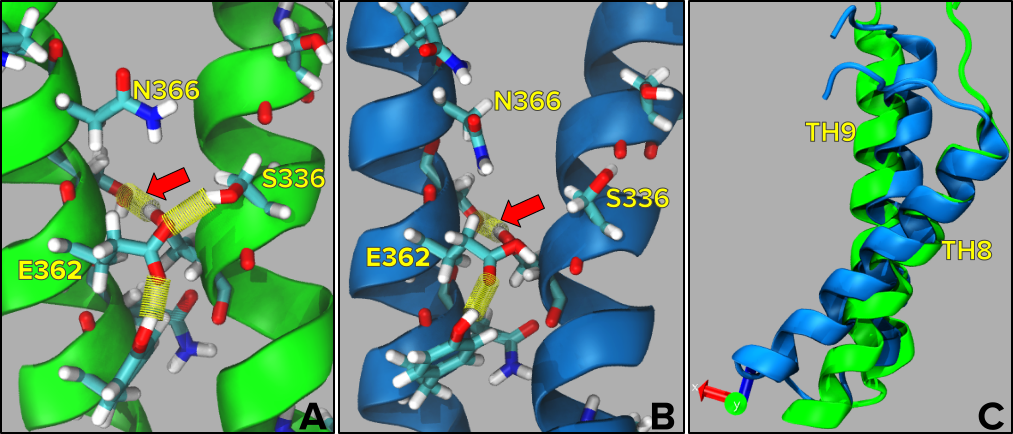
\includegraphics[width=\linewidth,]{Figures/DTT/hbonds_compare.png}
\caption[H-Bonds in DTT TH8-TH9 helices]{Hydrogen bond network between the TH8-TH9 helices involving residues S336, S337, E362, S363, and N366. The red arrow points to the H-bond formed between residues S337/S363 which are the two closest points of contacts between the helices. When E362 is charged (Fig.\ref{fig:dtt_hbonds}A; green), residues N366/S336 are oriented inward but are flipped away when E362 is neutral (Fig.\ref{fig:dtt_hbonds}B; blue). Fig. \ref{fig:dtt_hbonds}C shows the shift of the TH8 helix when E362 is charged by overlaying the protein structure from neutralized E362.}
\label{fig:dtt_hbonds}
\end{figure}

From our MD simulations, we found that the exposure of the charge on residue E362 within the membrane environment results in the two helices moving closer together to effectively shield the unfavorable charge in the center of the surrounding non-polar membrane environment. 
When residue E362 is charged, the two helices are pulled together by formation of a hydrogen bond network primarily involving residues surrounding E362.
From Figure \ref{fig:dtt_hbonds}, we show that resi- dues S336 and S337 on the TH8 helix are oriented inward in order to more closely interact with residues N366, S363, and charged E362 on the opposing TH9 helix.
From calculating the percent occupancy of hydrogen bond contacts between S336 and S363—the two closest residues on opposing helices-—we find that when residue E362 is neutral, hydrogen bonding occurs in roughly 57\% of trajectory frames, but when E362 is charged the hydrogen bonding occurs in approximately 88\% of the trajectory frames.
Our analysis of the MD trajectories indicates that when E362 is charged, the two helices are drawn closer together, thereby decreasing the overall perturbation to the membrane.
This finding suggests favorability for neutralized over charged E362 during the membrane insertion mechanism as formation of a larger pore could better facilitate delivery of the catalytic domain across the membrane.

\begin{table}[H]
\centering
\caption[Cross-sectional area of DTT pore]{Mean cross-sectional area along the Z-axis of the pore formed by DTT when E362 is charged versus neutral. Calculated from dxTuber\cite{raunest2011dxtuber}, using average solvent densities with average versus minimum protein densities.}
\label{tbl:dtt_pore}
\begin{tabular}{|c|c|c|}
\hline
\textbf{E362 State}  & \boldmath$Avg(\AA^{2})$ & \boldmath$Min(\AA^{2})$ \\ \hline
Neutral & 740 & 318 \\ \hline
Charged & 750 & 217 \\ \hline
\end{tabular}
\end{table}

\begin{figure}[H]
\centering
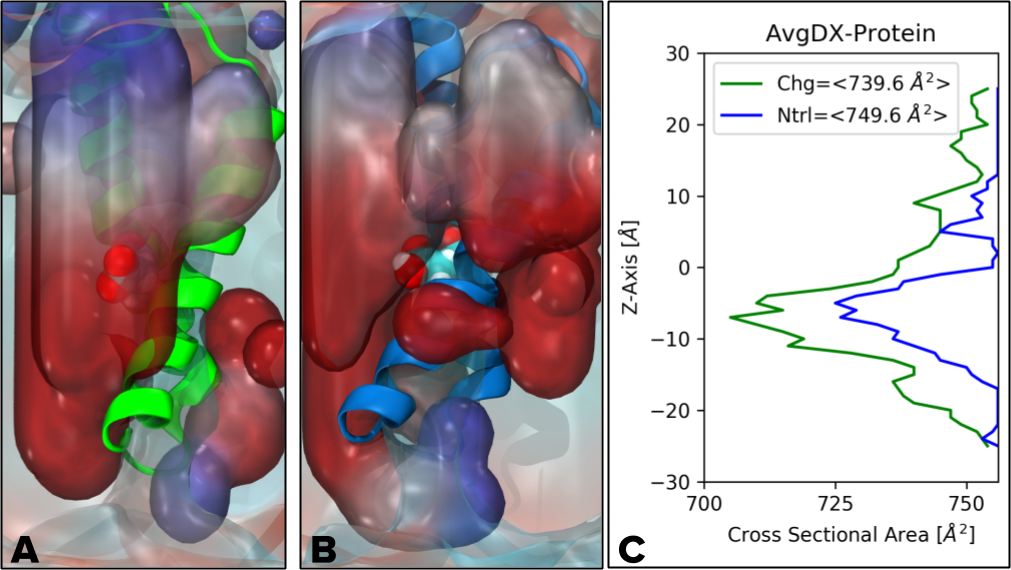
\includegraphics[width=\linewidth,]{Figures/DTT/avgdx.png}
\caption[Solvent accessibility of DTT pore]{Solvent accessibility map using average protein and average solvent densities over the 64ns MD simulation. The time-averaged solvent densities are shown for when E362 is charged (Fig.\ref{fig:dtt_avgdx}A; green) and when E362 is neutral (Fig.\ref{fig:dtt_avgdx}B; blue). Solvent densities are colored red for high density and blue for low density. Fig.\ref{fig:dtt_avgdx}C plots the cross-sectional area along the Z-axis with the mean cross-sectional areas being 750\AA$^2$ for neutral E362 and 740\AA$^2$ for charged E362 (Table \ref{tbl:dtt_pore}).}
\label{fig:dtt_avgdx}
\end{figure}

In order to approximate the pore size from T-domain insertion, we use dxTuber to calculate the cross-sectional area along the membrane normal over the course of the MD trajectories. 
By using the average protein and average solvent densities, we generate a time-averaged map of solvent accessibility around the protein (Fig.\ref{fig:dtt_avgdx}).
Solvent accessibility is colored by according to the averaged density (red=high density; blue=low).
From our analysis (Table \ref{tbl:dtt_pore}), we find that the average cross-sectional area when residue E362 is neutral is 750\AA$^2$ and when charged is 740\AA$^2$.
Next, by using the minimum protein densities with averaged solvent densities, we filter out regions of high protein flexibility.
This yields a map of the areas with maximum solvent accessibility, which appears to map the solvent accessibility of pore interior (Fig.\ref{fig:dtt_mindx}).
The average cross-sectional area through the inner cavity when residue E362 is neutral is 318\AA$^2$ and when charged is 217\AA$^2$.
Both the average and minimum protein profiles indicate the overall pore formed in the membrane by T-domain insertion is greater in size when residue E362 is neutralized.
This analysis provides further evidence that membrane perturba- tion starts with the initial insertion of TH8–9 domain and that E362 may play multiple roles in modulating the inser- tion mechanism of the T-domain.

\begin{figure}[H]
\centering
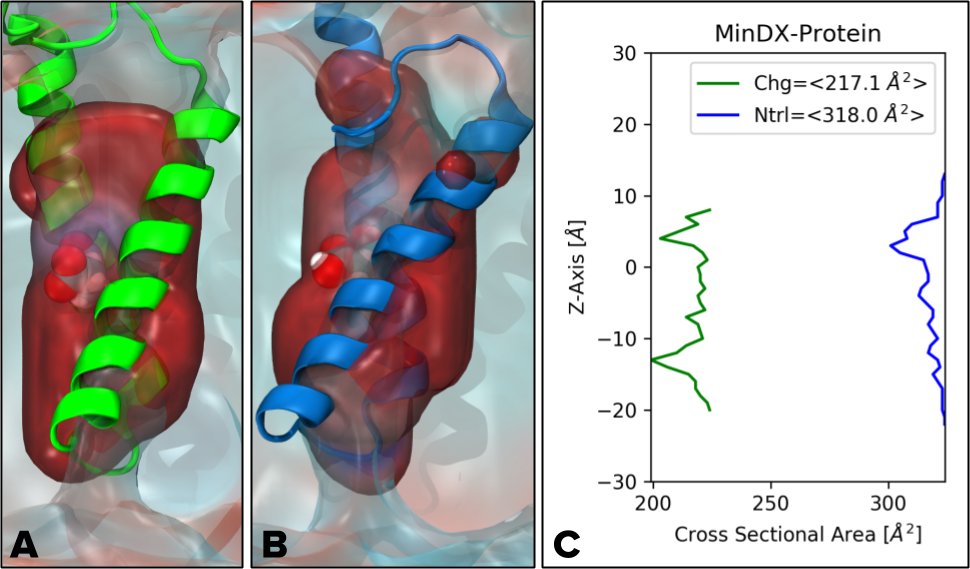
\includegraphics[width=\linewidth,]{Figures/DTT/mindx.png}
\caption[Solvent accesibility map for Charged E362 DTT Pore]{Maximum solvent accessibility map for when E362 is charged (Fig.\ref{fig:dtt_mindx}A; green) and neutral (Fig.\ref{fig:dtt_mindx}B; blue), using minimum protein and average solvent densities over the 64ns MD simulation. Fig.\ref{fig:dtt_mindx}C plots the cross-sectional area along the Z-axis with the mean cross-sectional areas being 318\AA$^2$ for neutral E362 and 217\AA$^2$ for charged E362 (Table \ref{tbl:dtt_pore}).}
\label{fig:dtt_mindx}
\end{figure}

\section{Summary}
In our alchemical free energy calculations, we alchemically transform the glutamic acid residue at position 362 from its charged to neutral state by effectively creating or annihilating a proton on the side chain atoms.
Our simulations use a previously constructed model of the full T domain (seq. 202-378) in aqueous solution with residue E362 charged, all histidine residues neutralized, and aspartic/glutamic acid residues ionized. 
Simulations involving the membrane use a partial T-domain model of just the TH8-TH9 helices (seq. 319-380) embedded into the membrane, where all histidine residues were ionized and aspartic/glutamic acid residues were neutralized.
These protonation states were as recommended by our experimental collaborators in view of the experimental data.

From our initial results, the free energy change calculated from alchemically creating a proton to neutralize the charged glutamic residue was $+84.4\frac{kcal}{mol}$ in the membrane and $+86.0\frac{kcal}{mol}$ in the aqueous environment, yielding an insertion free energy of $-1.6\frac{kcal}{mol}$.
This result indicates some favorability for the neutral state over the charged state in the membrane, by at least $1.6\frac{kcal}{mol}$.
However, this analysis neglects corrections to computed free energies due to finite-size effects.
After applying a correction scheme based off a thorough continuum-electrostatics analysis\cite{rocklin2013calculating}, we obtain a predicted final insertion free energy of $-6.2 (+/-0.4)\frac{kcal}{mol}$.

Here, the alchemical free energy calculations for the critical titratable residue E362 (\ref{fig:dtt_thermo_cycle}; \ref{tbl:dtt_ddG}) revealed a 6 kcal/mol difference favoring the membrane partitioning of the protonated form versus the ionized form, thus providing important thermodynamic insights into pH-triggered conformational switching during bilayer insertion.
Solvent accessibility calculations revealed that neutral form of E362 perturbs the integrity of the lipid bilayer (Figs. \ref{fig:dtt_avgdx}, \ref{fig:dtt_mindx}), providing atomistic insights into pH- dependent interactions of the T-domain with the lipid bilayer. 
Overall, the proposed methodology in this study, which combines MD simulations and free energy calculations, can be used for understanding thermodynamic details relevant to physiological action of a variety of bilayer-inserted proteins.